\section{实验原理}

\subsection{字母与置换表示}

本实验将 26 个英文字母按照 $A=0,B=1,\ldots,Z=25$ 编码。接线板、转子和反射器都可以看作字母集合上的置换。若一个部件将输入字母对应到输出字母，则可以用一个长度为 26 的数组表示该置换。

\subsection{Enigma机的加密结构}
\begin{figure}[H]
    \centering
    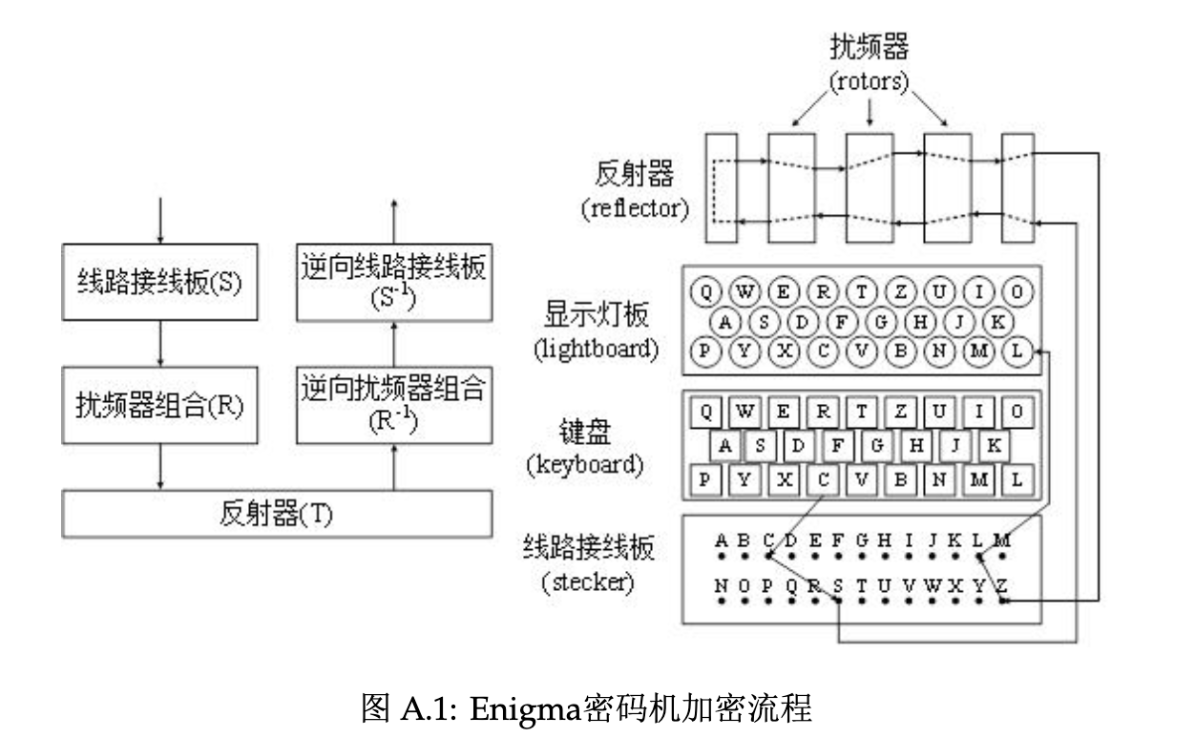
\includegraphics[width=0.8\textwidth]{figures/Enigma.png}
    \caption{Enigma机的结构}
    \label{fig:Enigma}
\end{figure}
Enigma 机主要由接线板、转子组和反射器组成。设接线板置换为 $S$，三个转子在当前状态下共同形成的正向变换为 $R_i$，反射器置换为 $T$。其中下标 $i$ 表示正在处理第 $i$ 个字符时的转子状态。

对于明文字符 $P_i$，其加密过程为：先经过接线板，再依次通过三个转子和反射器，随后沿相反方向通过三个转子的逆变换，最后再次经过接线板。因此有

\begin{equation*}
    C_i=S^{-1} \circ R_i^{-1} \circ T \circ R_i \circ S(P_i).
\end{equation*}

式中，$S^{-1}$ 表示接线板的逆置换，$R_i^{-1}$ 表示当前转子组的逆变换，$T$ 表示反射器。反射器满足$T(\alpha) = \beta,\alpha \neq \beta$,即反射器的输入与输出必然不相等。这导致了Enigma具有密文字母一定与明文字母不同的特点：
令
$$
C = E(P) = S^{-1} \circ R^{-1} \circ T \circ R \circ S(P)
$$
假设存在$P = E(P)$，代入上式可得:
$$
P = S^{-1} \circ R^{-1} \circ T \circ R \circ S(P) \Rightarrow \\
R \circ  S(P) = T \circ R \circ S(P)
$$
令$ R \circ S(P) = \gamma $，上式得到:
$$
\gamma = T(\gamma)
$$
这与反射器的定义相矛盾，因此假设不成立，不存在$P$使得$P = E(P)$，这一特殊事件是后续对Enigma机破解的一个利用点。

\subsection{接线板}

接线板密钥记为 $K_1$。每条接线连接两个不同字母，使两个字母互相交换；没有接线的字母映射到自身。若接线板恰好有 $l$ 条接线，先从 26 个字母中选出参与接线的 $2l$ 个字母，再将其两两配对，因此可能的接线板数量为

\begin{equation*}
    N_{K_1}(l)=\binom{26}{2l}\frac{(2l)!}{2^l l!}
    =\frac{26!}{(26-2l)!2^l l!}.
\end{equation*}

其中 $2^l$ 用于消除每条接线两端交换所造成的重复计数，$l!$ 用于消除不同接线之间排列顺序造成的重复计数。按照参考程序中“不超过 6 条接线”的限制，严格的接线板密钥数量为

\begin{equation*}
    N_{K_1,\leq 6}=\sum_{l=0}^{6}N_{K_1}(l)
    =105\,578\,918\,576\approx2^{36.62}.
\end{equation*}

若只取接线数量最大的情况 $l=6$ 进行数量级估计，则

\begin{equation*}
    N_{K_1}(6)=\frac{26!}{14!2^6 6!}
    =100\,391\,791\,500\approx2^{36.55}.
\end{equation*}

\subsection{转子组与转动规则}

转子内部的连线是预先固定的，但转子的安装顺序和起始位置会改变整体置换。在任务一中，三个转子的顺序固定为快速、中速、慢速转子 $(I,II,III)$，起始位置为 $(8,9,10)$。每处理一个明文字符后，快速转子向前转动一个位置；快速转子转满 26 次后，中速转子转动一个位置；中速转子转满 26 次后，慢速转子转动一个位置。

若三个转子的集合固定但顺序未知，则转子顺序有 $3!$ 种选择，每个转子的起始位置有 26 种选择，因此转子密钥数量为

\begin{equation*}
    N_{K_2}=3!\times26^3=105\,456\approx2^{16.69}.
\end{equation*}

实际使用的Enigma机中为了增大$K_2$的密钥空间，通常会从$t$个备选转子中选择$3$个，并按照一定初始化顺序组成实际在用的扰频器，此时该密钥的数量为:
\begin{equation*}
    N_{K_2}  =  P_t^3 \times 26^3
\end{equation*}

在任务三中，从 4 个转子中选择 3 个并安排到快速、中速、慢速三个位置

因此任务三的转子密钥数量为

\begin{equation*}
    N_{K_2}'=P_4^3\times26^3=421\,824\approx2^{18.69}.
\end{equation*}
